%
% File acl2017.tex
%
%% Based on the style files for ACL-2015, with some improvements
%%  taken from the NAACL-2016 style
%% Based on the style files for ACL-2014, which were, in turn,
%% based on ACL-2013, ACL-2012, ACL-2011, ACL-2010, ACL-IJCNLP-2009,
%% EACL-2009, IJCNLP-2008...
%% Based on the style files for EACL 2006 by 
%%e.agirre@ehu.es or Sergi.Balari@uab.es
%% and that of ACL 08 by Joakim Nivre and Noah Smith

\documentclass[11pt,a4paper]{article}
\usepackage[hyperref]{acl2017}
\usepackage{times}
\usepackage{latexsym}
\usepackage[pdftex]{graphicx}

\usepackage{url}

\aclfinalcopy % Uncomment this line for the final submission
%\def\aclpaperid{***} %  Enter the acl Paper ID here

%\setlength\titlebox{5cm}
% You can expand the titlebox if you need extra space
% to show all the authors. Please do not make the titlebox
% smaller than 5cm (the original size); we will check this
% in the camera-ready version and ask you to change it back.

\newcommand\BibTeX{B{\sc ib}\TeX}

\title{Final project report for the Natural Language Understanding Systems course}

\author{Federico Giuggioloni \\
  189662 \\
  {\tt federico.giuggioloni@studenti.unitn.it}}

\date{}

\begin{document}
\maketitle
\begin{abstract}
Through the usage of Finite State Transducers and all related tools a Spoken Dialogue System that allows queries to a movie database is provided. This report will detail all steps of development, comprising all the problems that popped up during the various phases.
The end result allows a visualization of the resulting data on screen, with additional information acquired through scraping.
\end{abstract}

\section{Introduction}
The first part of the project was all about the generation of a good enough model to allow concept tagging of new phrases related to the movie domain. \cite{openfst} \cite{opengrm}

Now that model is put to use in an actual user interaction setting, in which the user asks about movies and receives the required information in real time.

As the model is not perfect, some errors may happen. Some parts of the phrase are tagged with the wrong concept, or certain concepts are completely skipped. For this reason some kind of error recovery is required, filling in the missing information through interaction with the user himself.

\section{Threshold and hyper parameter settings}

\subsection{Thresholds}
Two thresholds are needed for both the concept tagging and the intent classifier:

Acceptance Threshold: above which the SLU or UC is accepted

Rejection Threshold: below which the SLU or UC is rejected, forcing the system to ask for the missing information	

Any case that falls between the two thresholds triggers a confirmation from the system (for example "Did you really mean the movie avatar"?).

For both thresholds the test file has been taken into consideration once transformed into one sentence per line format.
Both the Concept tagger and Utterance classifier were run on the entire dataset, providing in output a confidence in the tagging for each phrase.

In the SLU case, the acceptance threshold has been set to the mean of the first best confidence provided by the tagger. The mean was chosen because some mistakes in the tagging are expected, so the lower confidences can be seen as uncertain. The rejection threshold was initially set to the mean of the confidences of the first taggings containing at least a single span, but it ended up never being used. The information provided by the concept tagger, even in the worst scenarios, can be useful in helping the user reach the expected answer.

For the Utterance Classifier the acceptance threshold has been calculated in the same way, but also an intent-specific threshold has been calculated. The goal of this was to avoid having a few intents appear as certain even when completely wrong (in particular, the intent movie, which always has a high probability of being chosen because of it's prevalence in the dataset).
The rejection threshold for the Utterance Classifier was at first set to the minimum of the 1-best confidences, but then has been tweaked over time as testing went on to achieve better results.

\subsection{Number of best results to consider}
To decide the number of best confidences to retrieve and use from the classifier and the concept tagger the same test sentences used for threshold calculation were used. For the computation itself, the number has been set to an arbitrarily high number.

This gave me a list of confidences for each sentence.
By counting the number of confidences above a certain "significativity" level (set to 1) and then computing the mean of these numbers I got a decent estimate of the number of best taggings to consider (n set to 3).

For the classifier, this was run but then deemed to be useless: The classifier itself returns at most a number of results equal to the number of possible intents. This means that by setting the number of best predictions to exactly the number of possible intents it is possible to consider all intents in order of importance in cases of confusion. This will be further detailed in the dialogue structure section.

\subsection{ASR confidence integration}
Threshold calculation was done by assuming ASR confidence equal to one 1 (strings were certain) to allow usage of the test set sentences.

For each user request, the SLU and UC confidences are multiplied by the ASR confidence just before checking with the thresholds. This means that if the ASR is uncertain about the utterance, the system will ask more questions.

\section{Problems with the provided tools and classes}
\subsection{Out of memory errors}
FstPrintStrings has a problem which makes it necessary to have around 60GB of RAM for phrases of 15 words or longer. This made it hard to test any long phrases, as even phrases 10 words long run the risk of taking too long to run or simply crash the script.

The reason for this problem seems to be that instead of just providing in output the n-best paths with their weights, fstprintstrings simply prints out all possible paths in the FST, and then gives the output to the PHP script that is going to sort the results. Changing fstprintstrings to just print the n-best paths should fix this problem.

\subsection{SLU Parsing}
The SLU parsing provided by the SluResults class has an important flaw in a very specific case. Let's consider the phrase "Is Mark Hamill in Star Wars":

\begin{verbatim}
	Tagging:
	O B-movie.name I-movie.name
	O B-movie.name I-movie.name
\end{verbatim}

The expected result provided by SLU parsing is something like this:

\begin{verbatim}
	"movie.name" => "Mark Hamill"
	"movie.name" => "Star Wars"
\end{verbatim}

Of course, due to the use of associative arrays, this "Star Wars" ends up overwriting "Mark Hamill", making the dialog manager completely forget about the first span.

Having both spans is important because it allows the dialog manager to ask about whether or not it is a movie name.
To allow both spans to exist in the result set, a simple ID has been appended to the concept tag:

\begin{verbatim}
	"movie.name:0" => "Mark Hamill"
	"movie.name:1" => "Star Wars"
\end{verbatim}

These numbers are just used to allow multiple instances of the same concept to exist inside the resulting associative array. In any function that makes use of the concept tagging either as an index to a dictionary or to check for keywords inside user responses the ID is stripped from the concept.

\section{Project Structure}

The project is based off the OpenFST and OpenGRM utilities, adapted by the professor for use in PHP during lab sessions.

The provided PHP classes have been slightly modified to fix some minor problems, as explained in the previous sections.

The project is provided in the form of a website, in which all processing and dialogue management is done Server side.

\subsection{Client side}
The Client is only necessary in providing an interface for the user. It accepts requests both as text input written directly with a keyboard and using ASR to speak to the assistant.

On each request, as soon as a response is received, the answer is read out using Text To Speech. In addition, any related information is showed on the screen, for example a list of the movies released in 1999 with all the information contained in the databse integrated with additional bits from their IMDB link. Most requests to the server are fast enough to provide a quick answer, so no message is showed to the user until a response is received.

The system allows the user to barge-in by starting the ASR recognition phase as soon as the response is being read out. This is provided as a setting inside the client because using this with speakers runs the risk of the assistant "listening to himself".

\subsection{Server side}
The Server side does all the computation needed to understand the semantics of the user's utterance.

The main structure is made of a PHP file that handles incoming requests, and a DialogManager class that stores the current dialog state. The state in question is sent back and forth between server and client to simplify debugging by being able to repeat situations simply reusing the same state in the request.

All responses from the Server not only provide the generated response from the assistant, but also the current results from the database (if applicable) and any debug information related to the last request (for example, SLU and UC results and confidences).

There are four main function provided by the dialog manager, which are run on each response cycle.

\subsubsection{Generate an answer}
Based on the nature of the request, and the results from the database, a string response that will be read to the user is generated. This is made to sound as natural as possible, and contains some specific responses for the most probable questions. (For example, if asking 'tell me about the matrix', the assistant will respond with the more specific 'here is additional information on the matrix' instead of the generic response 'The movie of the matrix is the matrix').

\subsubsection{Generate a question}
Allows error recovery. This is called when the confidences are below the acceptance threshold. A question, made to sound as natural as possible, is generated based on all the missing or uncertain information in the current dialog state. All the slots are filled or confirmed one after the other, starting from the intent and then going over the SLU uncertainties. When trying to recover from UC and SLU errors, a method based on checking keywords inside the user's utterance is used. This allows the user to specify his intent, confirm acquired concepts, modify the wrong concepts and even ignore certain spans that were wrongly tagged. If the user is bored of the current exchange, or the system is so confused that it is not providing useful question, the user can ask a new question. If the question proves to be simple enough (both SLU and UC confidence over the acceptance threshold) then the new question is answered, before asking the user whether or not he wants to return to the previous conversation. Also, saying the very specific "I want to ask a new question" will reset the dialogue state.

\subsubsection{Check if all slots have been filled}
This is used to check whether or not a query can be run at the current state of the dialog. Once a request is run on the database, the dialog state is reset on the next cycle, allowing new requests from the user.

\subsubsection{Fill missing slots}
This is the main keywording part of the dialog manager. Based on the current asked question runs a wide range of regexes and matches on the user's utterance to try and fill in the missing values. Checks for confirmation of fields through the usage of an array of possible affirmative sentences, while the negation uses an array of negative sentences. Acts very similarly to a bot.

\subsection{Dialogue}
As was said before, the Dialogue itself is mostly handled by the DialogManager class.
At each request, a full cycle of prediction is run in multiple steps:

\begin{itemize}
\item Recovering the current state: The current state of the dialog is always sent by the Client on each request. An empty state means the conversation just started.
\item Run SLU and UC and store the confidences.
\item If the confidences are both high enough, simply fill in all slots.
\item Otherwise, if a confidence is uncertain, store current unsure value and ask the user for confirmation.
\item If a confidence is below the rejection level the information is thrown away.
\item Completely independent from the confidences is the "fill-in" step, in which a wide array of keyword and regex based matching on the user's utterance are used to better understand the current request. This is based on the current state of the dialogue, to always provide precedence to the classifier and concept tagger outcomes.
\item If all the slots have been filled, run the query and run the answer generator.
\item If some slots are missing, run the question generator.
\item In both cases, send back a response containing the next phrase that will be said by the assistant, with eventual results from the database and the current state of the dialogue. This last object will be the one that will be sent directly to the server on the next request.
\end{itemize}

The error recovery happens over multiple user requests, filling in one or more slots per utterance.

\subsection{Evaluation}

\subsubsection{Task based evaluation}
The generic task "obtain information about movies" has been taken into consideration, making all possible values of intents and concepts available.
Then 66 sentences were taken to run the system with and without error recovery. The results show an improvement on the number of times the system understands the sentence correctly.

\begin{figure}[h]
\centering
  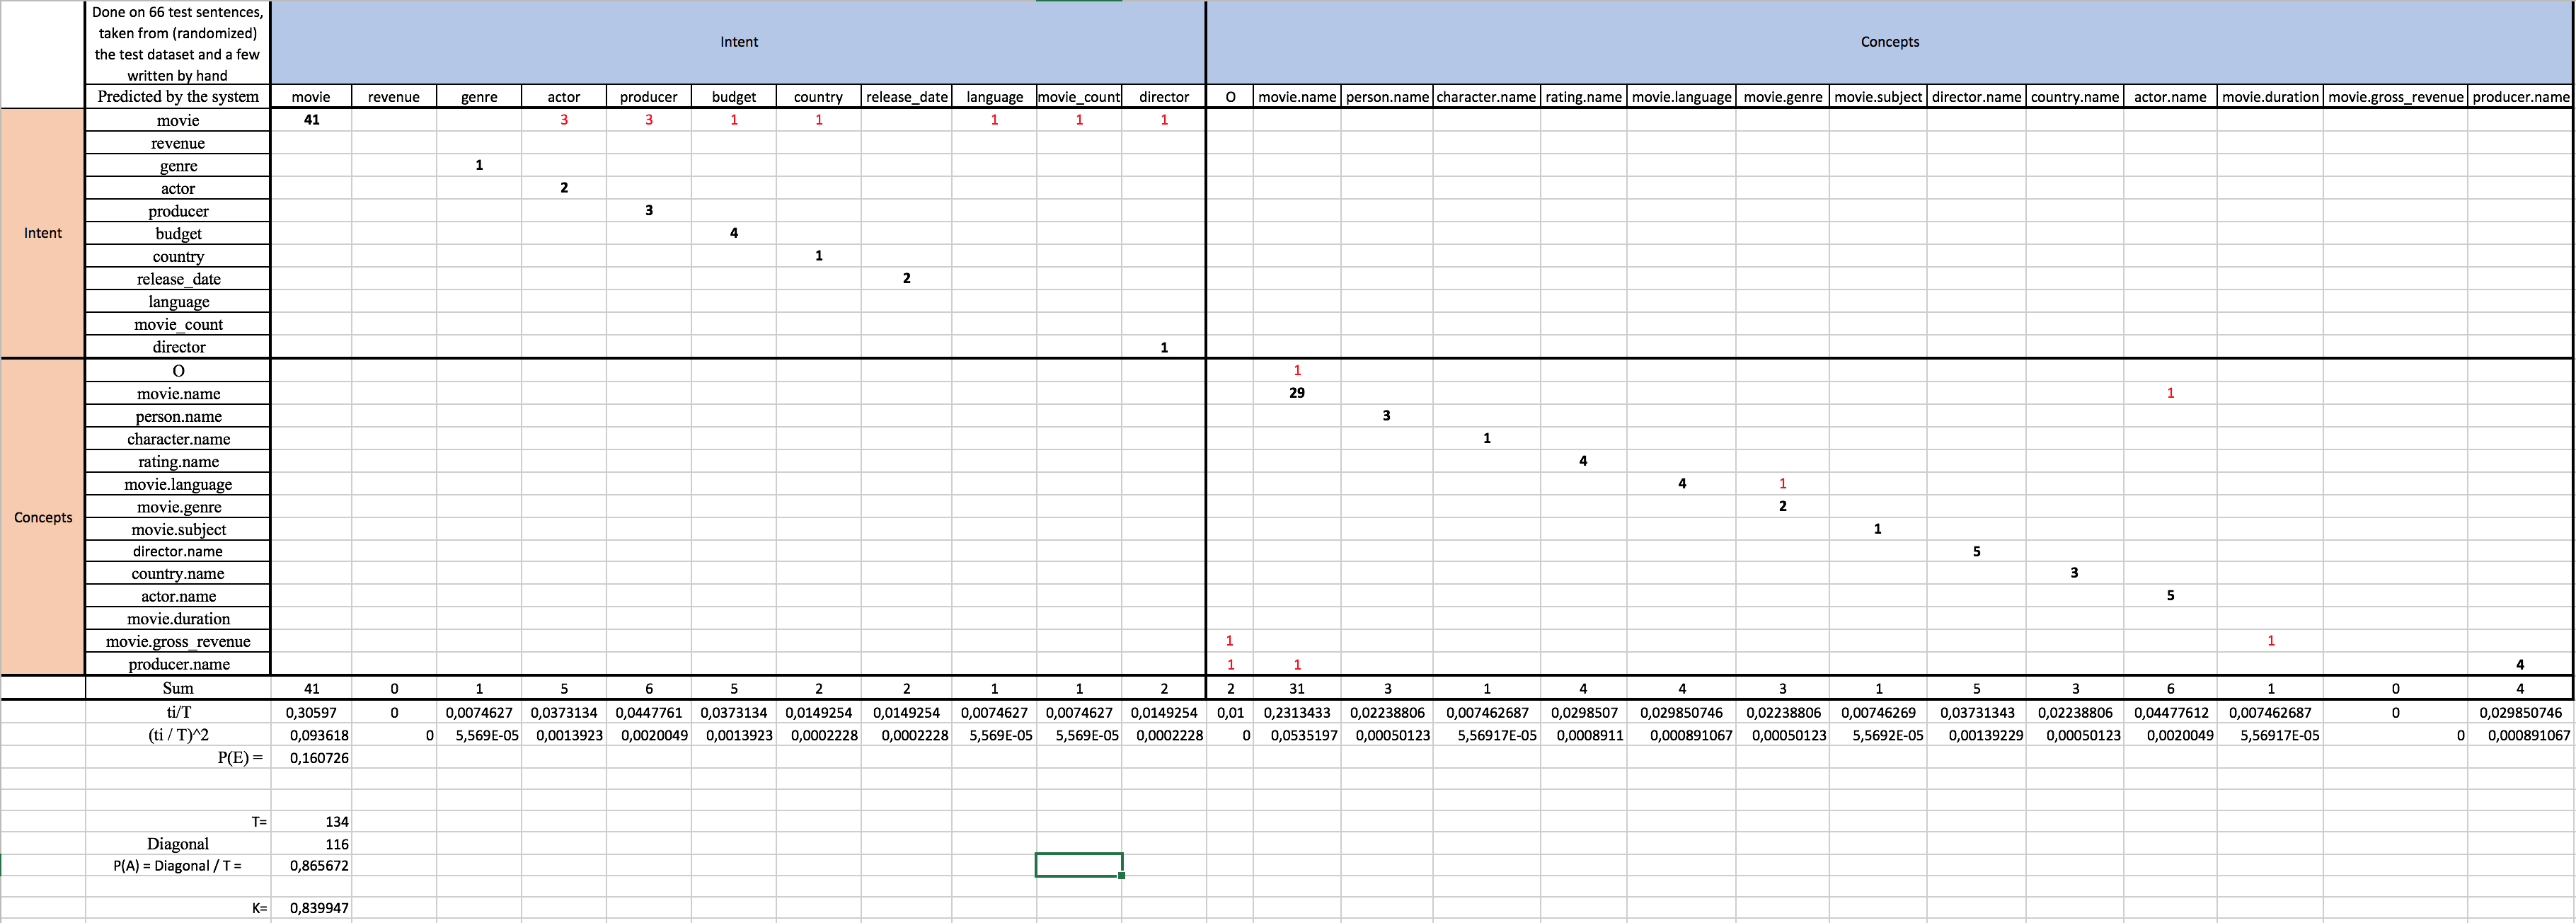
\includegraphics[width=.9\linewidth]{Images/noerrrec}
  \caption{Without error recovery}
\label{fig:zipf}
\end{figure}

\begin{figure}[h]
\centering
  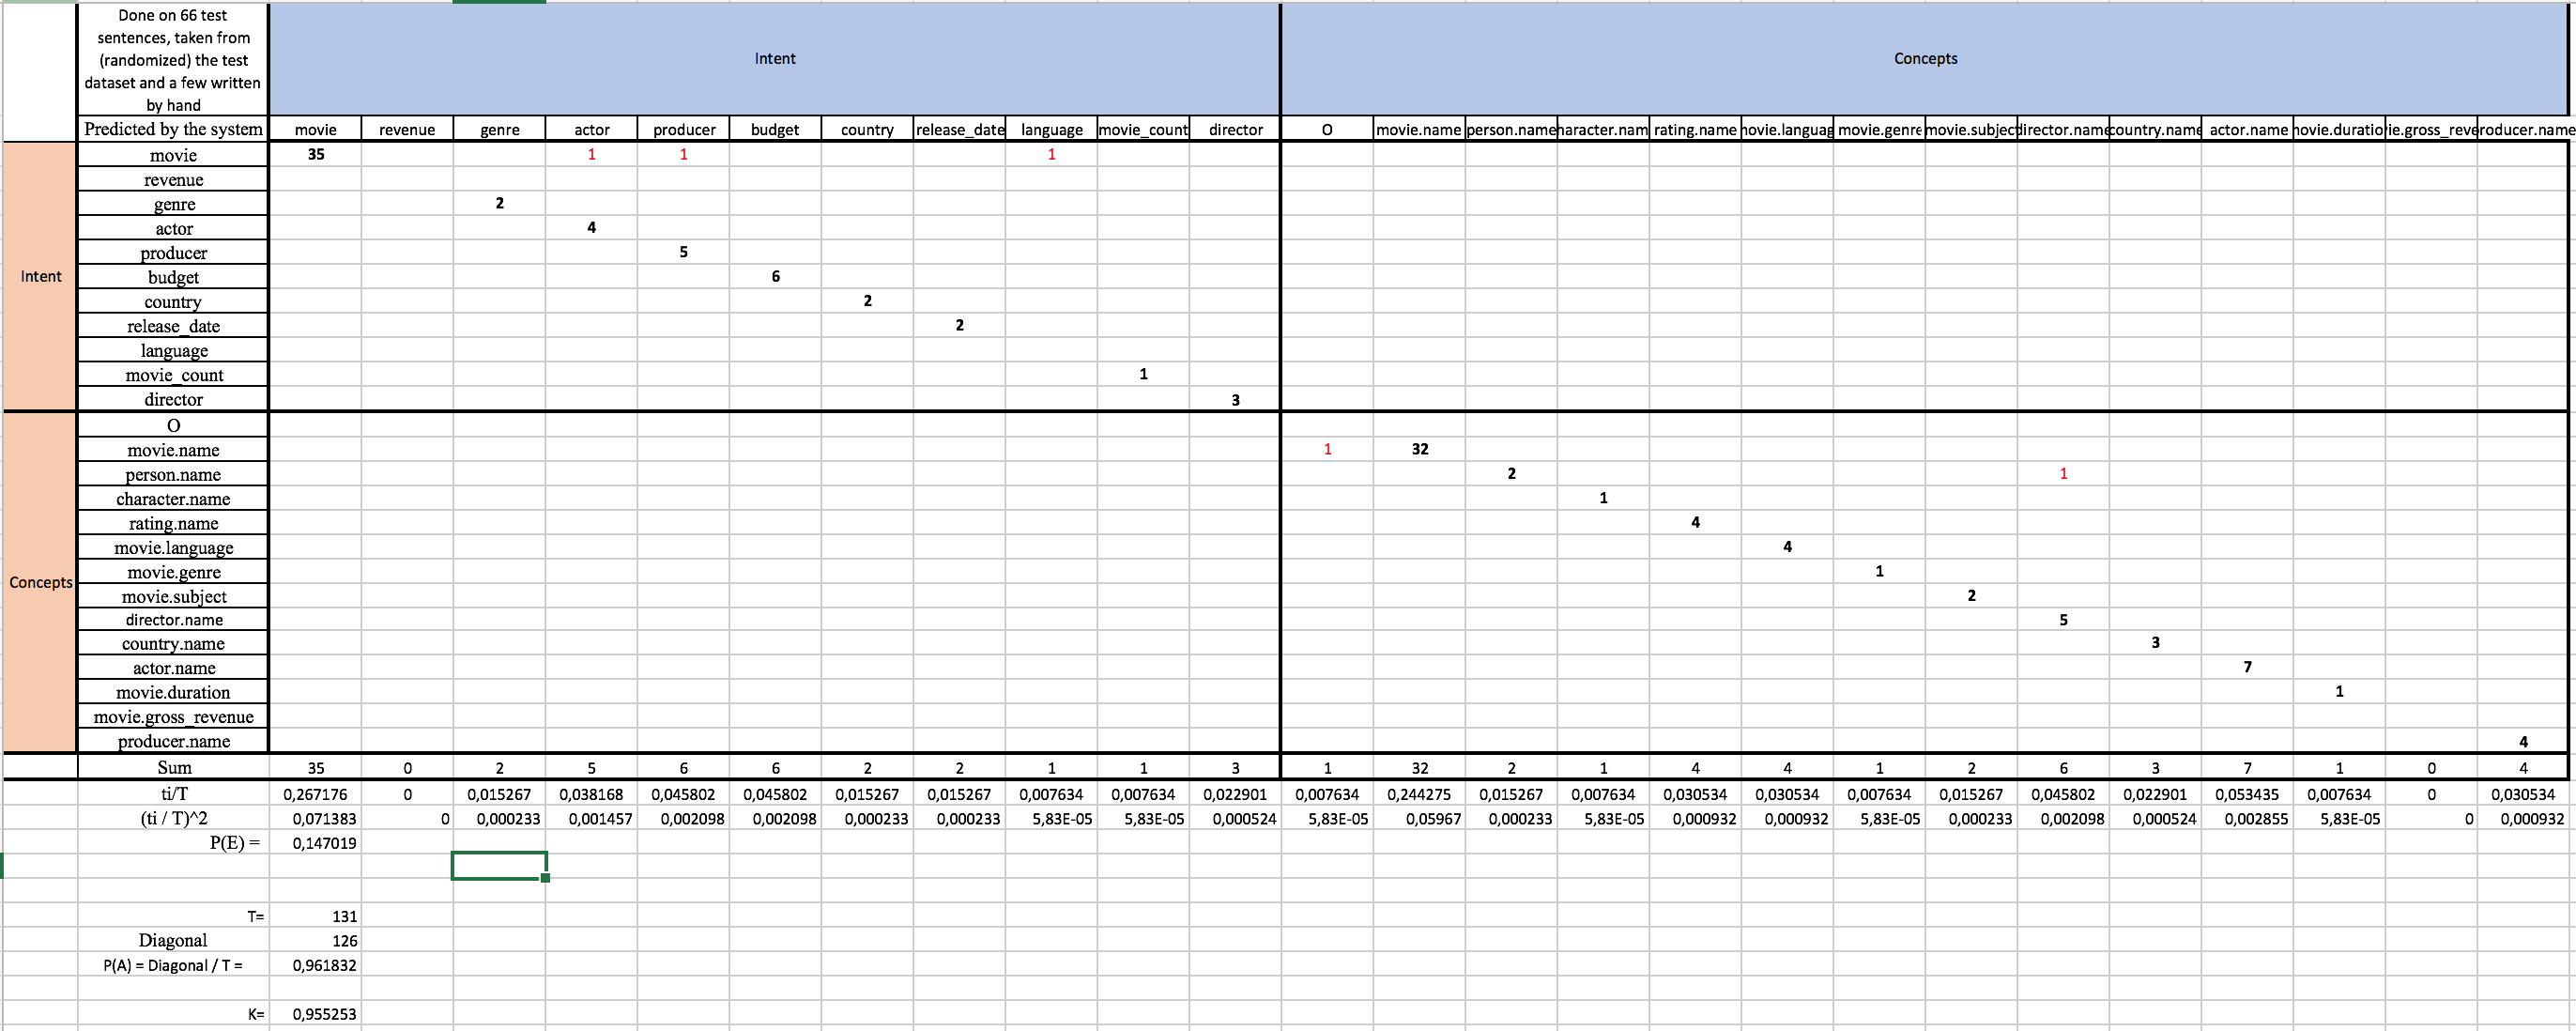
\includegraphics[width=.9\linewidth]{Images/errrec}
  \caption{With error recovery}
\label{fig:zipf}
\end{figure}

\section{Conclusions}
The system now contains a certain number of working features, and with the way it is built adding a new one is simple as long as the tags returned by the classifier and the concept tagger are enough to model it. In any other case a keyword based approach may be used for specific situations, otherwise the model would have to be retrained with different phrases and concept tags. 

In addition, the error recovery provided greatly improves the quality of the answers received by the system. A possible improvement could be that of shortening every interaction, as right now a lot of questions are asked. Improvements to the model may also lower the number of required questions.







% include your own bib file like this:
%\bibliographystyle{acl}
%\bibliography{acl2017}
\bibliography{acl2017}
\bibliographystyle{acl_natbib}

\appendix

\end{document}
